\documentclass[10pt]{book}

%-- imports
% QRK
\newcommand{\runDate}{202007}
\newcommand{\multipleNum}{7}
\newcommand{\projectNum}{9}
\newcommand{\iterationNumber}{1}

% Set Specific Variables
\newcommand{\setNumberStart}{0}
\newcommand{\setNumberEnd}{21}
\newcommand{\cardNumberStart}{7}
\newcommand{\cardNumberEnd}{7}

% Card Size
\newcommand{\cardHeight}{4}
\newcommand{\cardWidth}{5.5}

% Cropmarks with Paper Size
\newcommand{\cropPlusCardHeight}{101.6}%4} -101.6
\newcommand{\cropPlusCardWidth}{140} %5.5 - 152.4

% page dimensions
\newcommand{\halfHeight}{2.125} %1.9 for box!
\newcommand{\halfWidth}{2.75}  %2.8

% --- Packages
\usepackage[	%
						papersize={ 	\cropPlusCardWidth mm,	
											\cropPlusCardHeight mm},
						%papersize={,},
						topmargin = 5mm,
						%textheight = \cropPlusCardHeight mm,
						botmargin = 5mm,
						ytrim = 0mm,
						%
						leftmargin = 5mm,
						textwidth = \cropPlusCardWidth mm,
						rightmargin = 5mm,
						%
						cropmarks,
%						cropframe, 
						croplength = 5mm,
						cropgap= 2.5mm,
						nopagenumbers
					]{zwpagelayout}

\usepackage{tikz} 			%draw

\usepackage{fontspec}		%Set font
\setmainfont{Orbit}         % special by Evan Pittson Design. If you don't have this font, use something on your computer. Or comment out this line.

\usepackage{ifthen}			% if then else

\usepackage{mathtools}

% --- Formatting
\pagenumbering{gobble}
\setlength{\parindent}{0pt}


% --- Defined Values

% Constants
\newcommand{\altMargin}{1}
\newcommand{\lrMarginStart}{2.6}
\newcommand{\udMarginStart}{2}
\newcommand{\senderNAnchor}{1.4}
\newcommand{\recipientSAnchor}{-1.25}
\newcommand{\sendInstructionsX}{-2.6}
\newcommand{\sendInstructionsY}{1.35}
\newcommand{\recipInstructionsX}{2.5}
\newcommand{\recipInstructionsY}{-1.175}
% Card 19
\newcommand{\sendInsX}{-\lrMarginStart+1.25}
\newcommand{\sendInsY}{1.05}
\newcommand{\recipOneInsX}{\lrMarginStart-0.2}
\newcommand{\recipOneInsY}{-0.25}
\newcommand{\recipTwoInsX}{-.5}
\newcommand{\recipTwoInsY}{-0.75}

\newcommand{\sender}{Sender}
\newcommand{\recipient}{Recipient}


% Styling
\newcommand{ \cardTitleSty }[1]{\raggedright \large \MakeUppercase #1}
\newcommand{ \personSty }[1]{\raggedright \normalsize \MakeUppercase #1}
\newcommand{ \altPersonSty }[1]{\raggedright \tiny \MakeUppercase #1}
% Instructions
\newcommand{\instructionFormatting}[1]{\small \MakeLowercase #1}
\newcommand{\altInstructionFormatting}[1]{\tiny \MakeLowercase #1}


\begin{document}
	\newcommand{\card}{19}

	%\newcommand{\cardTitle}{collective memory}
%\newcommand{\instructionsOneS}{think of a memory shared by at least 2 others}
%\newcommand{\instructionsTwoS}{write your name and 2 others}
%\newcommand{\instructionsThreeS}{write about the memory}
%\newcommand{\instructionsOneR}{read about the memory}
%\newcommand{\instructionsTwoR}{add your thoughts about the memory}
%%\newcommand{\instructionsTwoROne}{send to the next recipient}
%\newcommand{\instructionsOneRTwo}{read and remember}

%
\newcommand{\cardTitle}{collective memory}
\newcommand{\instructionsOneS}{think of a shared memory}
\newcommand{\instructionsTwoS}{write your name and 2 others}
\newcommand{\instructionsThreeS}{write about the memory}
\newcommand{\instructionsOneR}{read about the memory}
\newcommand{\instructionsTwoR}{send to the next recipient}
	%Generate QRK Number
\newcommand{\qrkNumber}
  {QRK$\;$M$\multipleNum_{\iterationNumber}\;\runDate:
  \begin{matrix*}[l]
    \card \in  S_{\set}  | \{ \cardNumberStart, \dots , \cardNumberEnd\} = S_{\set}\\
    S_{\set} \subset \{ S_\setNumberStart, \dots , S_{\setNumberEnd}\}
  \end{matrix*}$}
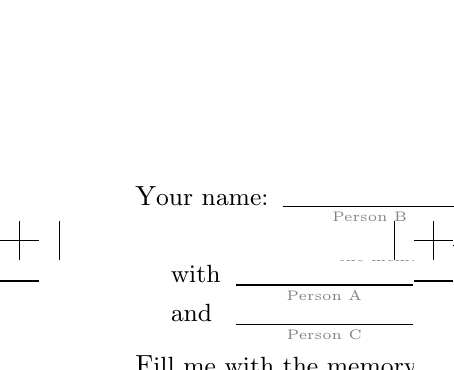
\begin{tikzpicture}[]

    	% title
    	\node[anchor=north west] at (-\lrMarginStart,\udMarginStart)
        { \cardTitleSty{\cardTitle}};

    	% QRK Number
    	\node[anchor=south west] at (-\lrMarginStart, -\udMarginStart)
        { \tiny \qrkNumber};

%    	% sender label
%    	\ifthenelse{\senderOn = 1}
%    					 % for the sender
%    					 {\node[anchor=north east, rotate = 90, text = black!50!white]
%                at (-\lrMarginStart,\senderNAnchor) {\personSty{\sender}};}
%    					 % not for sender
%    					 {\node[anchor=north east, rotate = 90, text = black!20!white]
%                at (-\lrMarginStart,\senderNAnchor) {\personSty{\sender}};}
%
%    	% recipient label
%    	\ifthenelse{\recipientOn = 1}
%    					 % for the recipient
%    					 {\node[anchor=north east, rotate = -90, text = black!50!white ]
%                at (\lrMarginStart,\recipientSAnchor) {\personSty{\recipient}};}
%    					 % not for recipient
%    					 {\node[anchor=north east, rotate = -90,xc ]
%               at (\lrMarginStart,\recipientSAnchor) {\personSty{\recipient}};}

    	% instructions - sender
    	\node[anchor= north west] at (\sendInstructionsX,\sendInstructionsY)
        {Y\instructionFormatting{our name:}};
        \draw (\sendInsX+0.75,\sendInsY-0.075) -- (\sendInsX+3,\sendInsY-0.075);
        \node[anchor= center] at (\sendInsX+3.15,\sendInsY-0.075)
        {\instructionFormatting{.}};
        \node[anchor= north,text = black!50!white] at (\sendInsX+1.85,\sendInsY-0.025)
        {\tiny{Person B}};


    	\node[anchor= north west] at (\sendInstructionsX,\sendInstructionsY-0.5)
        {R\instructionFormatting{emember}};
       	\draw (\sendInsX+0.65,\sendInsY-0.575) -- (\sendInsX+3.5,\sendInsY-0.575);
       	 \node[anchor= center] at (\sendInsX+3.65,\sendInsY-0.575)
        {\instructionFormatting{,}};
        \node[anchor= north,text = black!50!white] at (\sendInsX+2.075,\sendInsY-0.525)
        {\tiny{the memory}};


		\node[anchor= north west] at (\sendInstructionsX+0.45,\sendInstructionsY-1)
        {\instructionFormatting{with}} ;
		\draw (\sendInsX-0.3+0.45,\sendInsY-1.075) -- (\sendInsX+0.45+1.95,\sendInsY-1.075);
		\node[anchor= north,text = black!50!white] at (\sendInsX+1.275,\sendInsY-1.025)
        {\tiny{Person A}};

        \node[anchor= north west] at (\sendInstructionsX+0.45,\sendInstructionsY-1.5)
        {\instructionFormatting{and}};
      \draw (\sendInsX-0.3+0.45,\sendInsY-1.575) -- (\sendInsX+1.95+0.45,\sendInsY-1.575);
        \node[anchor= north west] at (\sendInsX+2+0.45,\sendInstructionsY-1.5)
        {\instructionFormatting{?}};
        \node[anchor= north,text = black!50!white] at (\sendInsX+1.275,\sendInsY-1.525)
        {\tiny{Person C}};


		\node[anchor= north west] at (\sendInstructionsX,\sendInstructionsY-2.15)
        {F\instructionFormatting{ill me with the memory.}} ;

\end{tikzpicture}

							
\end{document}
